\documentclass[a4paper]{article}

\usepackage{amsmath}
\usepackage{amsfonts}
\usepackage{graphicx}
\usepackage{enumerate}
\usepackage{SIunits}
\usepackage{hyperref}
\usepackage{anysize}
\usepackage{hyperref}

\marginsize{2.5cm}{2.5cm}{1.5cm}{1.5cm}

\graphicspath{{./images/}}

\title{Design of Digital Platforms}
\author{Steven Janssens, Pieter Maene en Kristof Mari\"en}
\date{\today}

\begin{document}
\maketitle

\section{Overall Architecture}

After having written a software implementation of the Montgomery algorithm in \textit{C}, the conclusion was that this was too slow for a real implementation. Therefore, in the second part of this course, we had to build a hardware coprocessor that should significantly increase speed. The final goal of this project was to build RSA encryption and decryption.\\

\begin{figure}[h]
	\center{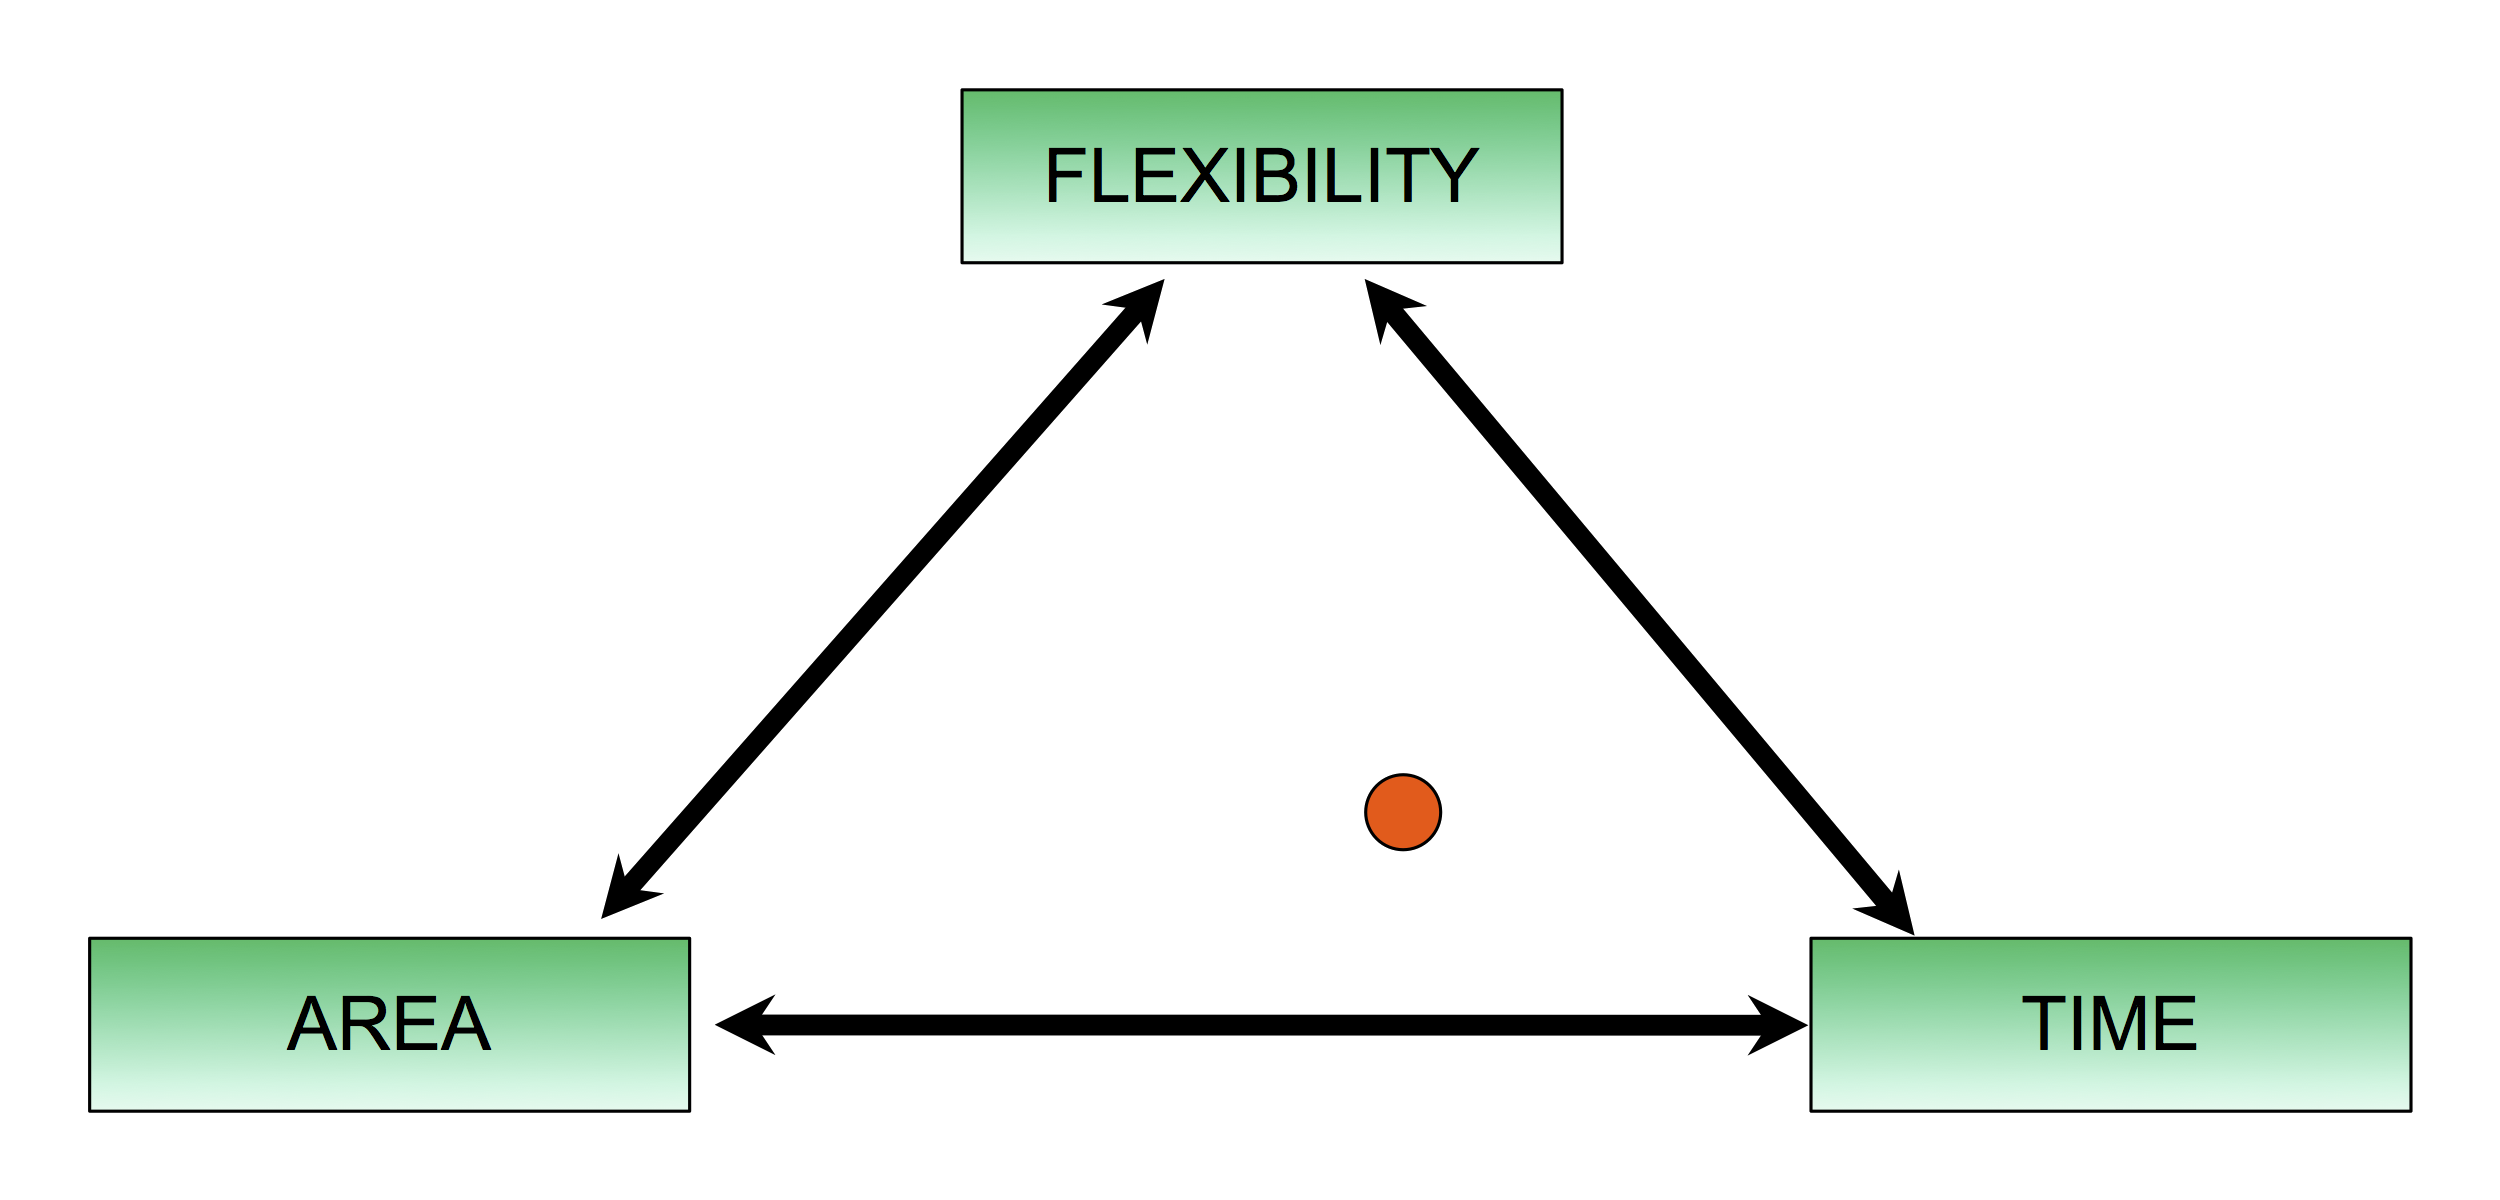
\includegraphics[width=0.8\linewidth]{situation.png}}
	\caption{Situation}
	\label{fig:situation}
\end{figure}

\section{HW/SW Boundaries}

The RSA algorithm is a basic and very often used algorithm for encryption and decryption of data. So it is important that the encryption and decryption is as fast as possible. The algorithm is standardized and will not change in the future. The only part of it that will change is the size of the inputs. Because of these facts we have chosen for a full hardware implementation.\\

From the previous section we know that a Montgomery multiplication takes about 1 second and a Montgomery exponentiation uses a lot of multiplications. So the multiplication must be done in hardware. Our hardware implementation takes about 1300 cycles. Assuming a clock frequency of about 5 \mega \hertz, this means a multiplication in hardware takes about 0,26 \micro \second.\\

So the only choice that was left, was to do the exponentiation in \textit{C} and call every time the Montgomery multiplication of the hardware. But doing this would cause a lot of overhead to transfer the data from the software to the hardware en back. So we decided to write the exponentation in \textit{Gezel} as well.

\section{HW/SW Interface}

\section{Performance Metrics}

\section{Synthesis Results}

\section{Test Strategy}

\end{document}
